Programming for SIEMENS Tecnomatix Process Simulate was initially desirable, as it exposes a Microsoft .NET Framework compatible API. 
This allows developers to choose any of the many .NET languages to create Process Simulate plugins, including but not limited to C\#, C++, F\#, Visual Basic, Iron Python. 
All the code in this work is written in C\#.

\section{Writing Plug-ins}
Any .NET assembly can be a Process Simulate plugin, as it only looks at the contents. 
A class library project is ideal for this as there is no benefit for any other project type. 
For Process Simulate to pick up the assembly, it should be located in \emph{DotNetCommands} or \emph{DotNetExternalApplications} directories and registered with the application. 
These directories and any following paths are relative to the programs installation directory. 
Typically this would be \cls{C:/Program Files/Tecnomatix 13.0/eMPower}, but might differ based on the user's choice at install-time.

To register an external application or a command with Process Simulate, we need to use a utility \emph{CommandReg.exe} which comes with the application. 
When you launch the program a dialog, similar to the one presented in Figure~\ref{fig:CommandReg}, will appear. 
In this dialog we select the compiled file, we want to load, pick the commands located in the assembly and choose a filename for the configuration XML file which will be newly created. 
This XML allows the settings to be moved between computers easily. \\

\begin{figure}[H]
    \caption{CommandReg Utility}
    \centering
    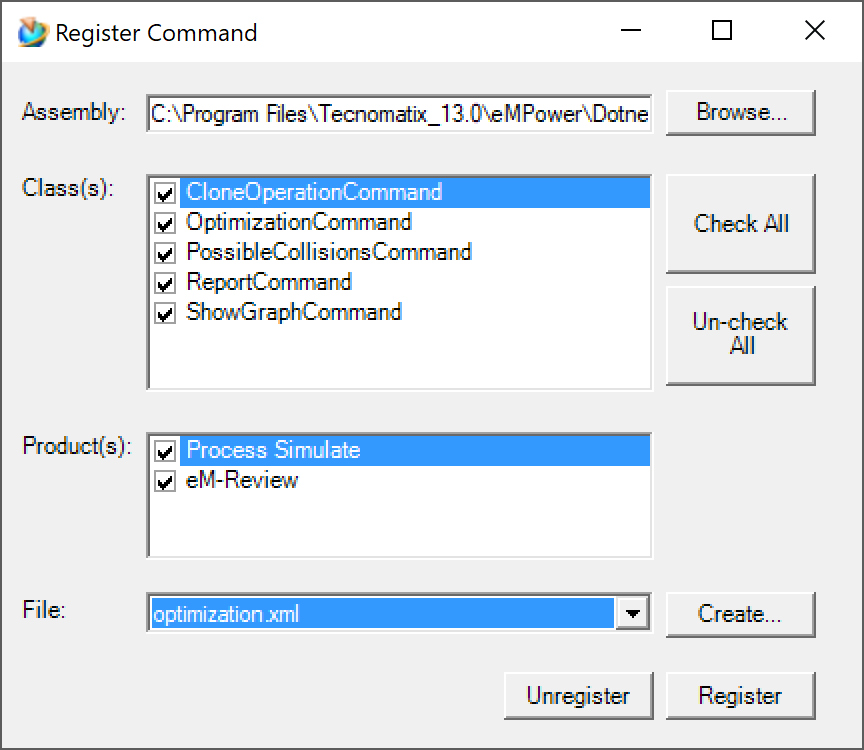
\includegraphics{commandreg}
    \label{fig:CommandReg}
\end{figure}

After we registered our commands, we need to configure our workspace to be able to use them. 
More specifically, we need to choose where the application should display buttons for the commands in the ribbon menu. 
This can be achieved by right-clicking the ribbon to invoke the context menu and selecting the \emph{Customize Ribbon} option as shown in Figure~\ref{fig:CustomizeRibbonContextMenu}.
A dialog like you see in Figure~\ref{fig:CustomizeRibbonDialog} will appear where the user can add new commands to the ribbon and customize the layout. 
The newly registered actions will appear in the list. Unfortunately, there is no grouping available. 
Therefore the best option is to look for the exact names in the alphabetically sorted list. \\

\begin{figure}[H]
    \caption{Customize the Ribbon}
    \centering
    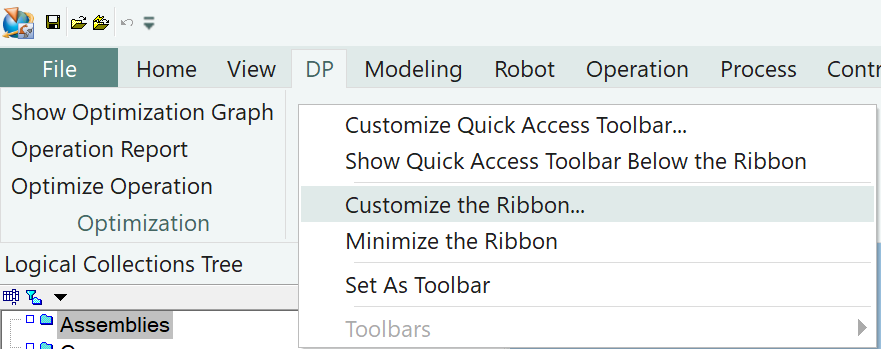
\includegraphics{customizeribbon}
    \label{fig:CustomizeRibbonContextMenu}
\end{figure}

\begin{figure}[H]
    \caption{Add commands to the Ribbon}
    \centering
    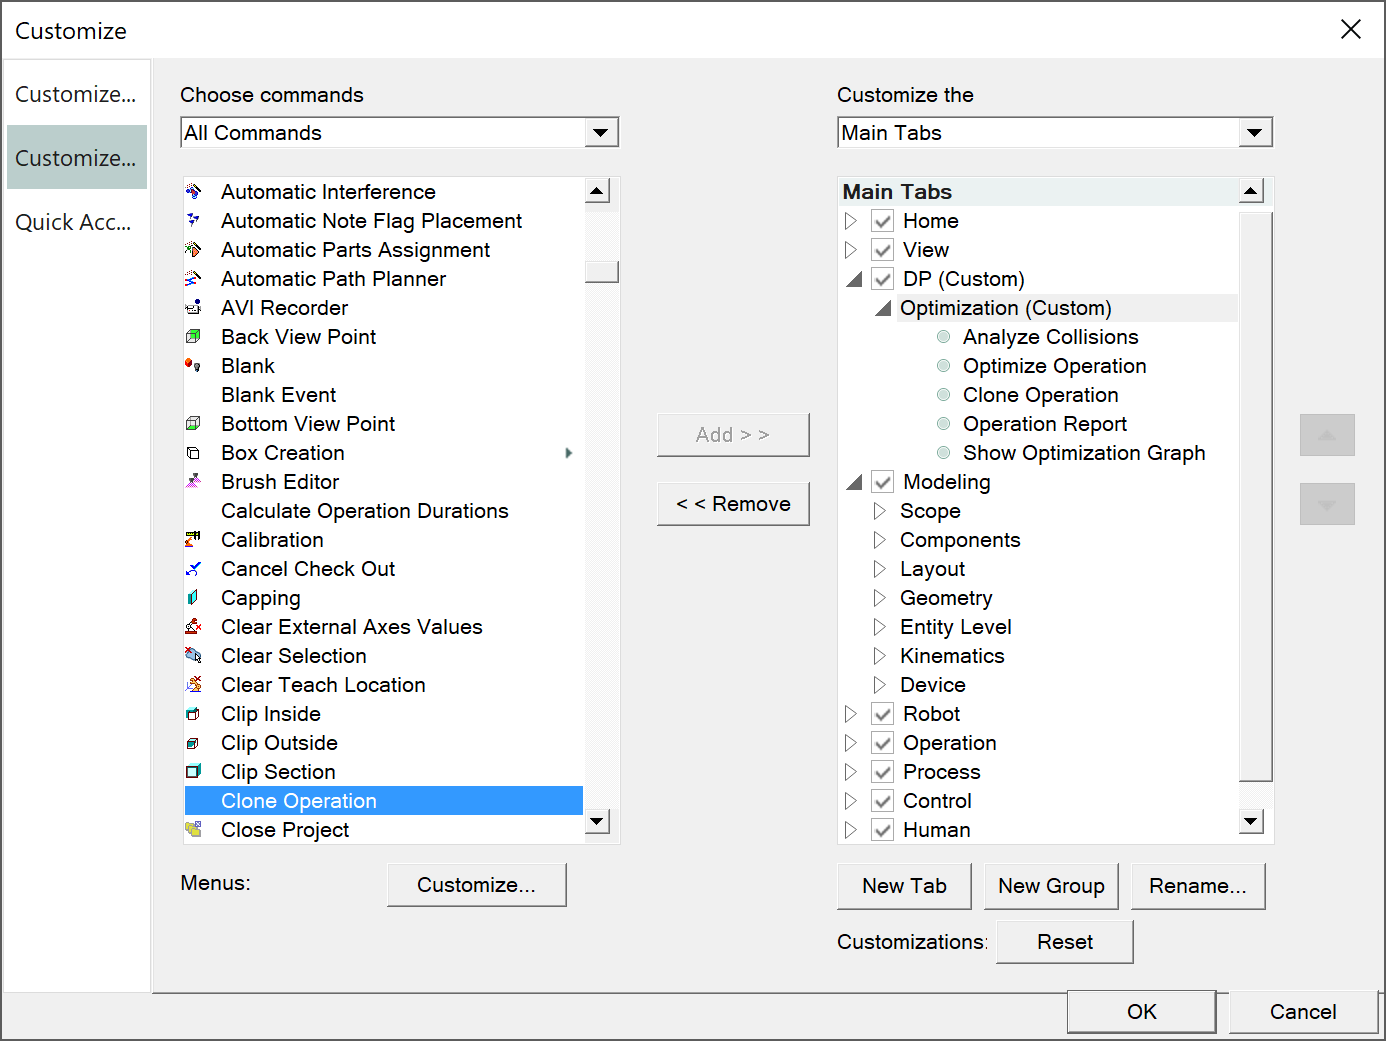
\includegraphics[width=\textwidth]{addcommands}
    \label{fig:CustomizeRibbonDialog}
\end{figure}

Next, we will look like at how to code new commands so that Process Simulate would recognize them. 
For this, we first need to include a reference for the main dynamically linked library \cls{Tecnomatix.Engineering.dll}. 
Writing plugins for the application revolves mostly around this one library, as it contains all the classes used to interact with the application. 
There are multiple types of commands which are recognized by Process Simulate.
They are named based on the UI elements they represent and range from buttons to combo boxes. 
Most commonly used command type is the button, which Figure~\ref{fig:CodeCommand} shows implemented.
To create a button command we have to create a new class and inherit the \cls{TxButtonCommand} abstract class.
After the user clicks the button, the \cls{Execute} method will be invoked, where we put our business logic. \\

\begin{figure}[H]
    \caption{Example Command}
    \centering
    \begin{minted}[breaklines]{csharp}
public class MyCommand : TxButtonCommand
{
    public override String Category { get; } = "My Category";
    public override String Name { get; } = "My Command";
    public override void Execute(Object cmdParams)
    {
    }
}
    \end{minted}
    \label{fig:CodeCommand}
\end{figure}

\section{API}

This section is dedicated to acquanting the reader with the most important classes in the \cls{Tecnomatix.Engineering.dll} library. 

\subsection{TxApplication}

The \cls{TxApplication} is a class containing static properties bound to the current application instance.
This is the main entry point the API.

\begin{figure}[H]
    \caption{TxApplication API}
    \centering
    \begin{minted}[breaklines]{csharp}
public sealed class TxApplication
{
    public static TxDocument ActiveDocument { get; }
    public static TxSelection ActiveSelection { get; }
    public static TxApplicationEvents ApplicationEvents { get; }
    public static TxOptions Options { get; }
    public static string StatusBarMessage { set; }
    public static void RefreshDisplay()
}
    \end{minted}
    \label{fig:CodeTxApplication}
\end{figure}

\cls{ActiveDocument} is the most important property of this object.
It contains information about the current document and allows applications to manipulate it.
See \cls{TxDocument}.

\cls{ActiveSelection} ... .

\cls{ApplicationEvents} property provides a way of getting a callback when the application is closing and so on.
See \cls{TxApplicationEvents}.

\cls{Options} contains a hierarchy of objects used to retrieve and set application options.
See \cls{TxOptions}.

\cls{StatusBarMessage} property can be used to relay status information to the user.
The text set to this property will appear on the application status bar.

For performance reasons, viewers may not always display the current data.
The method \cls{RefreshDisplay()} causes all viewers to display the current data.

\subsection{TxSelection}

\begin{figure}[H]
    \caption{TxSelection API}
    \centering
    \begin{minted}[breaklines]{csharp}
public sealed class TxSelection{
    public void Clear();
    public void AddItems(TxObjectList items);
    public void SetItems()
    public void RemoveItems()
    public ITxObject GetLastPickedItem();
    public TxTransformation GetLastPickedLocation();
    public TxObjectList GetPlanningItems();
    public TxObjectList GetAllItems();
    public TxObjectList GetOrderedItems();
    public event TxSelection_ItemsSetEventHandler ItemsSet;
    public event TxSelection_ItemsAddedEventHandler ItemsAdded;
    public event TxSelection_ItemsRemovedEventHandler ItemsRemoved;
}
    \end{minted}
    \label{fig:CodeTxSelection}
\end{figure}

\cls{GetOrderedItems()} gets the objects that are currently selected.
Returns only the loaded objects, in their engineering representation in the order they were selected in.
\cls{GetAllItems()} returns the same thing, but does not guarantee order.
\cls{GetPlanningItem()} returns planning representations like \cls{TxPlanningPart} or \cls{TxPlanningResource}, whereas \cls{GetAllItems()} returns engineering representations like \cls{TxRobot} or \cls{TxComponent}.


\cls{GetLastPickedLocation()} returns coordinates of the last picked object.


\subsection{TxApplicationEvents}

\begin{figure}[H]
    \caption{TxApplicationEvents API}
    \centering
    \begin{minted}[breaklines]{csharp}
public sealed class TxApplicationEvents
{
    public event TxApplication_ExitingEventHandler Exiting;
    public event TxApplication_ExitRequestEventHandler ExitRequest;
    public event TxApplication_ExitingEventHandler Closing;
}
    \end{minted}
    \label{fig:CodeTxApplicationEvents}
\end{figure}

\cls{Exiting} Occurs when the application is about to exit.

\cls{ExitRequest} Occurs when the application requests to exit.
To reject the request to exit, specify \cls{false} for the \cls{Approve} field of \cls{Tecnomatix.Engineering.TxApplication\_ExitRequestEventArgs}.

\cls{Closing} Occurs when the loaded project is closed.

Usage:

\begin{figure}[H]
    \caption{TxApplicationEvents Usage}
    \centering
    \begin{minted}[breaklines]{csharp}
private void Form1_Exiting(object sender, TxApplication_ExitingEventArgs args)
{
    FinishWork();
}
private void Form1_ExitRequest(object sender, TxApplication_ExitRequestEventArgs args)
{
    args.Approve = !working;
}
    \end{minted}
    \label{fig:CodeTxApplicationEventsUsage}
\end{figure}

\subsection{TxOptions}

Provides access to the application options as they are defined in the Options dialog.
These options include collision checking configuration, units used, simulation and so on.
Notably spot welding options aren't available in RobotExpert. 

Probably only option useful to plugins is:

\begin{figure}[H]
    \caption{TxOptions Usage}
    \centering
    \begin{minted}[breaklines]{csharp}
TxApplication.Options.Collision.StopOnCollision = true;
    \end{minted}
    \label{fig:CodeStopOnCollision}
\end{figure}


Which ensures the simulation player stops playing when it reaches the first collision.

\subsection{TxDocument}

The \cls{TxDocument} object is the common root of all model objects: physical
objects, operations, manufacturing features, and robotic programs. It provides
access to objects that have a single instance per document.

\begin{figure}[H]
    \caption{TxDocument API}
    \centering
    \begin{minted}{csharp}
public sealed class TxDocument
{
    public ITxOperation CurrentOperation { get; }
    public TxOperationRoot OperationRoot { get; }
    public TxPhysicalRoot PhysicalRoot { get; }
    public TxMfgRoot MfgRoot { get; }
    public TxCollisionRoot CollisionRoot { get; }
    public TxSimulationPlayer SimulationPlayer { get; }
}
    \end{minted}
    \label{fig:CodeTxDocument}
\end{figure}

\cls{OperationRoot} is the root of the operation tree
\cls{PhysicalRoot} is the root of the physical object tree
\cls{MfgRoot} is the root of the manufacturing features tree.

The \cls{ColisionRoot} is the root of the collision pairs.
It is used to determine where the workspace currently contains a colision.

The \cls{SimulationPlayer} is used to simulate operations and events.
At any given moment there is a single, current simulation player, with which all commands and viewers work.

\subsection{Operations}

\subsubsection{TxOperationRoot}

This class is the root of all operations.
Its children are usually of type \cls{TxCompoundOperation}.
You can query all children with the \cls{GetXDescendants()} methods.
Operations can't be created using a constructor.
To create a new operation use the \cls{CreateXOperation()} on a class that implements \cls{ITxOperationCreation} like \cls{TxOperationRoot}, for the specific operation type you are trying to create.
The created operation still needs to be inserted into a specific place in the operation tree.

\begin{figure}[H]
    \caption{TxOperationRoot API}
    \centering
    \begin{minted}[breaklines]{csharp}
bool CanCreateXOperation()
TxXOperation CreateXOperation(XCreationData creationData)
GetDirectDescendants(ITxTypeFilter filter)
GetAllDescendants(ITxTypeFilter filter)
//usage:
TxCompoundOperation newOperation =TxApplication.ActiveDocument.OperationRoot.CreateCompoundOperation(newTxCompoundOperationCreationData("name"));
foreach (ITxOperation op inTxApplication.ActiveDocument.OperationRoot.GetDirectDescendants(newTxNoTypeFilter()))
{
}
    \end{minted}
    \label{fig:CodeTxOperationRoot}
\end{figure}


\subsubsection{TxCompoundOperation}

Represents several operations grouped together into a single entity which together make a process.
This class implements is directly enumerable.
Like all operations compound operation has also a name and a description.

\begin{figure}[H]
    \caption{TxCompoundOperation API}
    \centering
    \begin{minted}{csharp}
TxCompoundOperation compoundOp = ...;
foreach (ITxOperation op in compoundOp)
{

}
    \end{minted}
    \label{fig:CodeTxCompoundOperation}
\end{figure}


\subsubsection{TxContinuousRoboticOperation}

Represents an ordered list of operations each with a certain duration that as a whole create a sequence that will be carried out by the robot.
Continuous robotic operation contains a set of child links, each having a reference to a from and to operations.
These links are read only but can be read and manipulated using the \cls{GetChildAt()} and \cls{MoveChildAfter()} functions.
Timing offsets and durations are read-only and can't even be changed in RobotExpert.

\begin{figure}[H]
    \caption{TxContinuousRoboticOperation API}
    \centering
    \begin{minted}[breaklines]{csharp}
TxContinuousRoboticOperation roboOp = ...;
IEnumerable<ITxOperation> children = Enumerable.Range(0, roboOp.Count)
    .Select(roboOp.GetChildAt)
    .OfType<ITxOperation>();
    \end{minted}
    \label{fig:CodeTxContinuousRoboticOperation}
\end{figure}

\subsubsection{TxRoboticViaLocationOperation}

This operation is used to avoid obstacles since a normal operation goes for a direct approach to the target point which can result in collisions.
Specifies a point to which the robots head should navigate.

\subsubsection{TxObjectFlowOperation}

This operation is used for moving products from one location to another.
The operation specifies how the object is supposed to be gripped with \cls{GripFrame} (=\cls{TxFrame}) and \cls{GripFrameType} (=\cls{GeometricCenter}) properties.
The product will be moved through points specified by objects of type \cls{TxObjectFlowLocationOperation} that are children of the operation (as \cls{IEnumerable}).
